%% infiPaper.tex
%% 2008/12/09
%% by Daniel Kirchner, Alex Lotz, Andreas Steck


\documentclass[11pt, journal]{IEEEtran}
%\documentclass[conference]{IEEEtran}
%
% If IEEEtran.cls has not been installed into the LaTeX system files,
% manually specify the path to it like:
% \documentclass[journal]{../sty/IEEEtran}


% Some very useful LaTeX packages include:
% (uncomment the ones you want to load)

%% this is to get centered captions (figure)
\makeatletter
\long\def\@makecaption#1#2{\ifx\@captype\@IEEEtablestring%
\footnotesize\begin{center}{\normalfont\footnotesize #1}\\
{\normalfont\footnotesize\scshape #2}\end{center}%
\@IEEEtablecaptionsepspace
\else
\@IEEEfigurecaptionsepspace
\setbox\@tempboxa\hbox{\normalfont\footnotesize {#1.}~~ #2}%
\ifdim \wd\@tempboxa >\hsize%
\setbox\@tempboxa\hbox{\normalfont\footnotesize {#1.}~~ }%
\parbox[t]{\hsize}{\normalfont\footnotesize \noindent\unhbox\@tempboxa#2}%
\else
\hbox to\hsize{\normalfont\footnotesize\hfil\box\@tempboxa\hfil}\fi\fi}
\makeatother


% *** MISC UTILITY PACKAGES ***
%
%\usepackage{ifpdf}
% Heiko Oberdiek's ifpdf.sty is very useful if you need conditional
% compilation based on whether the output is pdf or dvi.
% usage:
% \ifpdf
%   % pdf code
% \else
%   % dvi code
% \fi
% The latest version of ifpdf.sty can be obtained from:
% http://www.ctan.org/tex-archive/macros/latex/contrib/oberdiek/
% Also, note that IEEEtran.cls V1.7 and later provides a builtin
% \ifCLASSINFOpdf conditional that works the same way.
% When switching from latex to pdflatex and vice-versa, the compiler may
% have to be run twice to clear warning/error messages.


% *** CITATION PACKAGES ***
%
\usepackage{cite}
% cite.sty was written by Donald Arseneau
% V1.6 and later of IEEEtran pre-defines the format of the cite.sty package
% \cite{} output to follow that of IEEE. Loading the cite package will
% result in citation numbers being automatically sorted and properly
% "compressed/ranged". e.g., [1], [9], [2], [7], [5], [6] without using
% cite.sty will become [1], [2], [5]--[7], [9] using cite.sty. cite.sty's
% \cite will automatically add leading space, if needed. Use cite.sty's
% noadjust option (cite.sty V3.8 and later) if you want to turn this off.
% cite.sty is already installed on most LaTeX systems. Be sure and use
% version 4.0 (2003-05-27) and later if using hyperref.sty. cite.sty does
% not currently provide for hyperlinked citations.
% The latest version can be obtained at:
% http://www.ctan.org/tex-archive/macros/latex/contrib/cite/
% The documentation is contained in the cite.sty file itself.


% *** GRAPHICS RELATED PACKAGES ***
%
\ifCLASSINFOpdf
  \usepackage[pdftex]{graphicx}
  % declare the path(s) where your graphic files are
  % \graphicspath{{../pdf/}{../jpeg/}}
  % and their extensions so you won't have to specify these with
  % every instance of \includegraphics
  % \DeclareGraphicsExtensions{.pdf,.jpeg,.png}
\else
  % or other class option (dvipsone, dvipdf, if not using dvips). graphicx
  % will default to the driver specified in the system graphics.cfg if no
  % driver is specified.
  % \usepackage[dvips]{graphicx}
  % declare the path(s) where your graphic files are
  % \graphicspath{{../eps/}}
  % and their extensions so you won't have to specify these with
  % every instance of \includegraphics
  % \DeclareGraphicsExtensions{.eps}
\fi
% graphicx was written by David Carlisle and Sebastian Rahtz. It is
% required if you want graphics, photos, etc. graphicx.sty is already
% installed on most LaTeX systems. The latest version and documentation can
% be obtained at: 
% http://www.ctan.org/tex-archive/macros/latex/required/graphics/
% Another good source of documentation is "Using Imported Graphics in
% LaTeX2e" by Keith Reckdahl which can be found as epslatex.ps or
% epslatex.pdf at: http://www.ctan.org/tex-archive/info/
%
% latex, and pdflatex in dvi mode, support graphics in encapsulated
% postscript (.eps) format. pdflatex in pdf mode supports graphics
% in .pdf, .jpeg, .png and .mps (metapost) formats. Users should ensure
% that all non-photo figures use a vector format (.eps, .pdf, .mps) and
% not a bitmapped formats (.jpeg, .png). IEEE frowns on bitmapped formats
% which can result in "jaggedy"/blurry rendering of lines and letters as
% well as large increases in file sizes.
%
% You can find documentation about the pdfTeX application at:
% http://www.tug.org/applications/pdftex


% *** MATH PACKAGES ***
%
%\usepackage[cmex10]{amsmath}
% A popular package from the American Mathematical Society that provides
% many useful and powerful commands for dealing with mathematics. If using
% it, be sure to load this package with the cmex10 option to ensure that
% only type 1 fonts will utilized at all point sizes. Without this option,
% it is possible that some math symbols, particularly those within
% footnotes, will be rendered in bitmap form which will result in a
% document that can not be IEEE Xplore compliant!
%
% Also, note that the amsmath package sets \interdisplaylinepenalty to 10000
% thus preventing page breaks from occurring within multiline equations. Use:
%\interdisplaylinepenalty=2500
% after loading amsmath to restore such page breaks as IEEEtran.cls normally
% does. amsmath.sty is already installed on most LaTeX systems. The latest
% version and documentation can be obtained at:
% http://www.ctan.org/tex-archive/macros/latex/required/amslatex/math/


% *** SPECIALIZED LIST PACKAGES ***
%
%\usepackage{algorithmic}
% algorithmic.sty was written by Peter Williams and Rogerio Brito.
% This package provides an algorithmic environment fo describing algorithms.
% You can use the algorithmic environment in-text or within a figure
% environment to provide for a floating algorithm. Do NOT use the algorithm
% floating environment provided by algorithm.sty (by the same authors) or
% algorithm2e.sty (by Christophe Fiorio) as IEEE does not use dedicated
% algorithm float types and packages that provide these will not provide
% correct IEEE style captions. The latest version and documentation of
% algorithmic.sty can be obtained at:
% http://www.ctan.org/tex-archive/macros/latex/contrib/algorithms/
% There is also a support site at:
% http://algorithms.berlios.de/index.html
% Also of interest may be the (relatively newer and more customizable)
% algorithmicx.sty package by Szasz Janos:
% http://www.ctan.org/tex-archive/macros/latex/contrib/algorithmicx/


% *** ALIGNMENT PACKAGES ***
%
%\usepackage{array}
% Frank Mittelbach's and David Carlisle's array.sty patches and improves
% the standard LaTeX2e array and tabular environments to provide better
% appearance and additional user controls. As the default LaTeX2e table
% generation code is lacking to the point of almost being broken with
% respect to the quality of the end results, all users are strongly
% advised to use an enhanced (at the very least that provided by array.sty)
% set of table tools. array.sty is already installed on most systems. The
% latest version and documentation can be obtained at:
% http://www.ctan.org/tex-archive/macros/latex/required/tools/


%\usepackage{mdwmath}
%\usepackage{mdwtab}
% Also highly recommended is Mark Wooding's extremely powerful MDW tools,
% especially mdwmath.sty and mdwtab.sty which are used to format equations
% and tables, respectively. The MDWtools set is already installed on most
% LaTeX systems. The lastest version and documentation is available at:
% http://www.ctan.org/tex-archive/macros/latex/contrib/mdwtools/


% IEEEtran contains the IEEEeqnarray family of commands that can be used to
% generate multiline equations as well as matrices, tables, etc., of high
% quality.


%\usepackage{eqparbox}
% Also of notable interest is Scott Pakin's eqparbox package for creating
% (automatically sized) equal width boxes - aka "natural width parboxes".
% Available at:
% http://www.ctan.org/tex-archive/macros/latex/contrib/eqparbox/


% *** SUBFIGURE PACKAGES ***
\usepackage[tight,footnotesize]{subfigure}
% subfigure.sty was written by Steven Douglas Cochran. This package makes it
% easy to put subfigures in your figures. e.g., "Figure 1a and 1b". For IEEE
% work, it is a good idea to load it with the tight package option to reduce
% the amount of white space around the subfigures. subfigure.sty is already
% installed on most LaTeX systems. The latest version and documentation can
% be obtained at:
% http://www.ctan.org/tex-archive/obsolete/macros/latex/contrib/subfigure/
% subfigure.sty has been superceeded by subfig.sty.


%\usepackage[caption=false]{caption}
%\usepackage[font=footnotesize]{subfig}
% subfig.sty, also written by Steven Douglas Cochran, is the modern
% replacement for subfigure.sty. However, subfig.sty requires and
% automatically loads Axel Sommerfeldt's caption.sty which will override
% IEEEtran.cls handling of captions and this will result in nonIEEE style
% figure/table captions. To prevent this problem, be sure and preload
% caption.sty with its "caption=false" package option. This is will preserve
% IEEEtran.cls handing of captions. Version 1.3 (2005/06/28) and later 
% (recommended due to many improvements over 1.2) of subfig.sty supports
% the caption=false option directly:
%\usepackage[caption=false,font=footnotesize]{subfig}
%
% The latest version and documentation can be obtained at:
% http://www.ctan.org/tex-archive/macros/latex/contrib/subfig/
% The latest version and documentation of caption.sty can be obtained at:
% http://www.ctan.org/tex-archive/macros/latex/contrib/caption/


% *** FLOAT PACKAGES ***
%
%\usepackage{fixltx2e}
% fixltx2e, the successor to the earlier fix2col.sty, was written by
% Frank Mittelbach and David Carlisle. This package corrects a few problems
% in the LaTeX2e kernel, the most notable of which is that in current
% LaTeX2e releases, the ordering of single and double column floats is not
% guaranteed to be preserved. Thus, an unpatched LaTeX2e can allow a
% single column figure to be placed prior to an earlier double column
% figure. The latest version and documentation can be found at:
% http://www.ctan.org/tex-archive/macros/latex/base/


%\usepackage{stfloats}
% stfloats.sty was written by Sigitas Tolusis. This package gives LaTeX2e
% the ability to do double column floats at the bottom of the page as well
% as the top. (e.g., "\begin{figure*}[!b]" is not normally possible in
% LaTeX2e). It also provides a command:
%\fnbelowfloat
% to enable the placement of footnotes below bottom floats (the standard
% LaTeX2e kernel puts them above bottom floats). This is an invasive package
% which rewrites many portions of the LaTeX2e float routines. It may not work
% with other packages that modify the LaTeX2e float routines. The latest
% version and documentation can be obtained at:
% http://www.ctan.org/tex-archive/macros/latex/contrib/sttools/
% Documentation is contained in the stfloats.sty comments as well as in the
% presfull.pdf file. Do not use the stfloats baselinefloat ability as IEEE
% does not allow \baselineskip to stretch. Authors submitting work to the
% IEEE should note that IEEE rarely uses double column equations and
% that authors should try to avoid such use. Do not be tempted to use the
% cuted.sty or midfloat.sty packages (also by Sigitas Tolusis) as IEEE does
% not format its papers in such ways.


%\ifCLASSOPTIONcaptionsoff
%  \usepackage[nomarkers]{endfloat}
% \let\MYoriglatexcaption\caption
% \renewcommand{\caption}[2][\relax]{\MYoriglatexcaption[#2]{#2}}
%\fi
% endfloat.sty was written by James Darrell McCauley and Jeff Goldberg.
% This package may be useful when used in conjunction with IEEEtran.cls'
% captionsoff option. Some IEEE journals/societies require that submissions
% have lists of figures/tables at the end of the paper and that
% figures/tables without any captions are placed on a page by themselves at
% the end of the document. If needed, the draftcls IEEEtran class option or
% \CLASSINPUTbaselinestretch interface can be used to increase the line
% spacing as well. Be sure and use the nomarkers option of endfloat to
% prevent endfloat from "marking" where the figures would have been placed
% in the text. The two hack lines of code above are a slight modification of
% that suggested by in the endfloat docs (section 8.3.1) to ensure that
% the full captions always appear in the list of figures/tables - even if
% the user used the short optional argument of \caption[]{}.
% IEEE papers do not typically make use of \caption[]'s optional argument,
% so this should not be an issue. A similar trick can be used to disable
% captions of packages such as subfig.sty that lack options to turn off
% the subcaptions:
% For subfig.sty:
% \let\MYorigsubfloat\subfloat
% \renewcommand{\subfloat}[2][\relax]{\MYorigsubfloat[]{#2}}
% For subfigure.sty:
% \let\MYorigsubfigure\subfigure
% \renewcommand{\subfigure}[2][\relax]{\MYorigsubfigure[]{#2}}
% However, the above trick will not work if both optional arguments of
% the \subfloat/subfig command are used. Furthermore, there needs to be a
% description of each subfigure *somewhere* and endfloat does not add
% subfigure captions to its list of figures. Thus, the best approach is to
% avoid the use of subfigure captions (many IEEE journals avoid them anyway)
% and instead reference/explain all the subfigures within the main caption.
% The latest version of endfloat.sty and its documentation can obtained at:
% http://www.ctan.org/tex-archive/macros/latex/contrib/endfloat/
%
% The IEEEtran \ifCLASSOPTIONcaptionsoff conditional can also be used
% later in the document, say, to conditionally put the References on a 
% page by themselves.


% *** PDF, URL AND HYPERLINK PACKAGES ***
%
\usepackage{url}
% url.sty was written by Donald Arseneau. It provides better support for
% handling and breaking URLs. url.sty is already installed on most LaTeX
% systems. The latest version can be obtained at:
% http://www.ctan.org/tex-archive/macros/latex/contrib/misc/
% Read the url.sty source comments for usage information. Basically,
% \url{my_url_here}.


% *** Do not adjust lengths that control margins, column widths, etc. ***
% *** Do not use packages that alter fonts (such as pslatex).         ***
% There should be no need to do such things with IEEEtran.cls V1.6 and later.
% (Unless specifically asked to do so by the journal or conference you plan
% to submit to, of course. )



% correct bad hyphenation here
\hyphenation{op-tical net-works semi-conduc-tor}

\begin{document}
%
% paper title
% can use linebreaks \\ within to get better formatting as desired
\title{Fatal Police Shootings in the USA}
%
%
% author names and IEEE memberships
% note positions of commas and nonbreaking spaces ( ~ ) LaTeX will not break
% a structure at a ~ so this keeps an author's name from being broken across
% two lines.
% use \thanks{} to gain access to the first footnote area
% a separate \thanks must be used for each paragraph as LaTeX2e's \thanks
% was not built to handle multiple paragraphs
%

\author{ \parbox{3 in}{\centering Andrei Martins, Daniel Dedoukh, Hidayat Rzayev, Ivaylo Gatev, Spyridon Ntokos\\
				 University of Applied Sciences Ulm\\
         {\tt\small {martins}@mail.hs-ulm.de, {dedoukh}@mail.hs-ulm.de, {ryazev}@mail.hs-ulm.de, {gatev}@mail.hs-ulm.de, {ntokos}@mail.hs-ulm.de}}
}


% The paper headers
\markboth{ }{A Template Paper}


% If you want to put a publisher's ID mark on the page you can do it like
% this:
%\IEEEpubid{0000--0000/00\$00.00~\copyright~2007 IEEE}
% Remember, if you use this you must call \IEEEpubidadjcol in the second
% column for its text to clear the IEEEpubid mark.

% use for special paper notices
%\IEEEspecialpapernotice{(Invited Paper)}




% make the title area
\maketitle

%%%%%%%%%%%%%%%%%%%%%%%%%%%%%%%%%%%%%%%%%%%%%%%%%%%%%%%%%%%%%%%%%%%%%%%%%%%%%%%%%%%%%%%%%%%%%%%%%%%%%%%%%%%%%%%%%%%%%%%%%%%%%%%%
%%%%%%%%%%%%%%%%%%%%%%%%%%%%%%%%%%%%%%%%%%%%%%%%%%%%%%%%%%%%%%%%%%%%%%%%%%%%%%%%%%%%%%%%%%%%%%%%%%%%%%%%%%%%%%%%%%%%%%%%%%%%%%%%
\begin{abstract}
Our project is based on CRISP-DM Model. After finding the proper datasets for our project, we went to the Business Understanding phase, where we defined the goals and critetia for our project. The main goal is to show how different aspects are related to the killings by the USA police. In Data Understanding and Data Preparation phases we inspected the data and applied Data Cleansing. After all the data has been prepared and harmonized, we created the CDWH with the dimensions and a fact table. For analytical purposes, we created a Data Mart out of our CDWH and performed the analysis. The key findings of the analysis are the amount of killings based on race, weapon, time, location and age.
\end{abstract}

% For peerreview papers, this IEEEtran command inserts a page break and
% creates the second title. It will be ignored for other modes.
%\IEEEpeerreviewmaketitle

%%%%%%%%%%%%%%%%%%%%%%%%%%%%%%%%%%%%%%%%%%%%%%%%%%%%%%%%%%%%%%%%%%%%%%%%%%%%%%%%%%%%%%%%%%%%%%%%%%%%%%%%%%%%%%%%%%%%%%%%%%%%%%%%
%%%%%%%%%%%%%%%%%%%%%%%%%%%%%%%%%%%%%%%%%%%%%%%%%%%%%%%%%%%%%%%%%%%%%%%%%%%%%%%%%%%%%%%%%%%%%%%%%%%%%%%%%%%%%%%%%%%%%%%%%%%%%%%%
\section{Introduction}
\label{sec:intro}
\subsection{Scenario} \label{subsec:scenario}
Our goal in this  project report is to show how social conditions as race, gender, income and others are related to the killings caused by the police in the USA. By analysing the data, we found patterns on how these killings are distributed among the population.

To achieve our objective of getting insightful meaning from the data, we will follow the
\emph{CRISP-DM process}  \cite{wikicrispdm}. Our main resources are 7 csv files that contain the data to be analysed. This data will be harmonized through the Staging Area before being inserted into the Database. The main tools used during the process where phpMyAdmin, MYSQL Workbench
and RStudio.

\subsection{Structure of the Paper} \label{subsec:struct}
The paper is structured as follows: in Section~\ref{sec:dataunderstanding} the process of extraction of the datasets is described.
Then, in Section~\ref{sec:datapreparation} the Staging Area and the data harmonization is detailed.  Section~\ref{sec:concept} describes how the Database was created, its dimensions and how they were combined for the Data Mart. In Section~\ref{sec:analytics} we show the relationship between the different data and some of graphics that represent these relationships visually. Finally, we conclude our work in Section~\ref{sec:concl} with the result of our analysis and what meaningful information we could get from it.

%%%%%%%%%%%%%%%%%%%%%%%%%%%%%%%%%%%%%%%%%%%%%%%%%%%%%%%%%%%%%%%%%%%%%%%%%%%%%%%%%%%%%%%%%%%%%%%%%%%%%%%%%%%%%%%%%%%%%%%%%%%%%%%%

\section{Open Data: Police Shootings in the US} \label{sec:dataunderstanding}
As part of the \emph{Data Understanding} phase for this data science project, the two available data sources are described: The CSV file \emph{PoliceKillingsUS}, taken from \cite{kaggle} contains the shootings that happened between years 2015 to 2017. There are four additional CSV files from that data source, which contain US census data on poverty rate, high school graduation rate, median household income, and racial demographics. The second CSV file, \emph{Police Fatalities} \cite{dataworld} contains data on fatalities dating back to 2000 up to year 2016.

%%%%%%%%%%%%%%%%%%%%%%%%%%%%%%%%%%%%%%%%%%%%%%%%%%%%%%%%%%%%%%%%%%%%%%%%%%%%%%%%%%%%%%%%%%%%%%%%%%%%%%%%%%%%%%%%%%%%%%%%%%%%%%%%

\section{Data Preparation} \label{sec:datapreparation}
The first step of the data preparation phase is extracting the data from our initial data sources and importing it into 2 MySQL databases, one for each datasets. This is a straightforward process, as we had to write one LOAD DATA statement for each of the .csv files, with the correct field and line termination symbols. For each field, we assigned an appropriate data type, as well as an appropriate primary key for each table. 
\begin{enumerate}
\item Police Fatalities Staging Area - The main tables(containing information about the police fatalities)  from our 2 datasets have a similar structure, with only a slight difference in the columns. We selected only the fields, which are relevant for our analysis and are available in both of the datasets. But despite all of this, the representation of some of the data is a little different. For example the values for race and gender are represented with their full names in one of the datasets, and with only the first letter in the other. Our strategy of dealing with this problem is deciding on one particular format for each field and storing the data in this unified way in the staging area. To avoid lower/upper case conflicts, we saved string values in upper case letters only. There are also some null values, which were automatically replaced by the LOAD DATA statement with an empty string for the VARCHAR type or 0 for numeric types. We stored the empty strings as ‘UNKNOWN’ in the staging area and kept the 0 as our value, which represents the unknown state, for the numeric types.

To harmonize the datasets we first stored the data for each one into a temporary table, applying the transformations described  previously. However, some duplicate values existed in the bigger dataset, as well as matching values between both of them. The problem is that not all of the duplicates are exact matches. For example 2 records contain the same values for all but one column, in particular for the columns race, weapon and age. One record would contain a concrete value for one particular field and the other one an unknown value. Naturally, we kept the record that contains more information about the fatality. 

Mostly there were only 2 duplicate rows for one fatality, but there were a few cases with 3 duplicates, which we dealt with manually. After that, we deleted the records that match ones from the smaller dataset. In the end, the temporary tables were merged into one. To make the ids more consistent, we dropped the original id columns and created our own auto increment primary key. Later, while working on the location dimension, we noticed that there was a typo in one of the records with the city Albuquerque and fixed it manually.

\begin{figure}[htb]
	\centering
		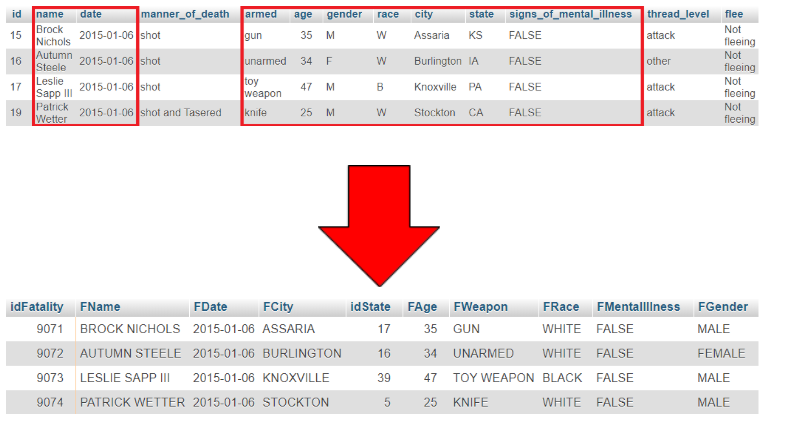
\includegraphics[width=1.0\columnwidth]{images/snapshot}
	\caption{Overview of solution strategy}
	\label{fig:probov}
\end{figure}

\item Age and Weapon  Maping Area - The Age Maping consist of the table MapAgeGroup.  The age groups were defined by an interval with an appropriate lower and upper bound(age group ‘UNKNOWN’ for 0 values). 

 For the Weapon Dimension, there are ~70 distinct weapons used in our staging area ’s ‘Fatality’ table. Using a “CASE WHEN … THEN …” SQL syntax, we ‘ve classified them in 10 distinct categories. This mapping table was stored in an intermediate database together with the Age maping tables.

\end{enumerate}

%%%%%%%%%%%%%%%%%%%%%%%%%%%%%%%%%%%%%%%%%%%%%%%%%%%%%%%%%%%%%%%%%%%%%%%%%%%%%%%%%%%%%%%%%%%%%%%%%%%%%%%%%%%%%%%%%%%%%%%%%%%%%%%%

\section{Concept for CDWH} \label{sec:concept}
The CDWH approach is visualized in Figure \ref{fig:probov2}.


\begin{enumerate}
	\item Time Dimension - The script used for the time dimension tables is a simplified version of the script written by Prof. Dr. Markus Goldstein. A procedure is used to build the calendar for days, months and year.
	\item MentalIllnes dimension - A True / False value is used to determine the mental state of the victim.
	\item Race dimension - Describes which race the victim belonged to. The values are: white, black, hispanic, native, asian, other or unknown.
	\item Gender dimension - Describes the gender of the victim: male, female or unknown.
	\item Weapon Dimension - Consisted of two tables, namely “Weapon” and “WeaponClass” which were populated according to the weapon mapping table from an intermediate database, with auto-increment IDs. Unknown weapon is declared as “UNKNOWN”.
	\item Age Dimension - The Age Dimension consists of the tables Age and Age Group. The age groups from the mapping table, without the lower and upper bound, were copied into the CDWH Age Group table. For the Age table, all of the distinct age values were taken from 			the staging area, mapped to their appropriate age group and inserted into the Age table of the CDWH. The age values themselves are used as a primary key to the table.
	\item Location Dimension - consists of the tables City and State. Since the states were available in the Staging Area, they were simply copied from there. The distinct cities were taken from the Fatalities table of the Staging Area, as well as various statistics for each city, such as poverty level, median household income, etc. were taken from one of the initial data sources. Cities, for which statistics was not available, are denoted with 0 values.

\end{enumerate}

\begin{figure}[htb]
	\centering
		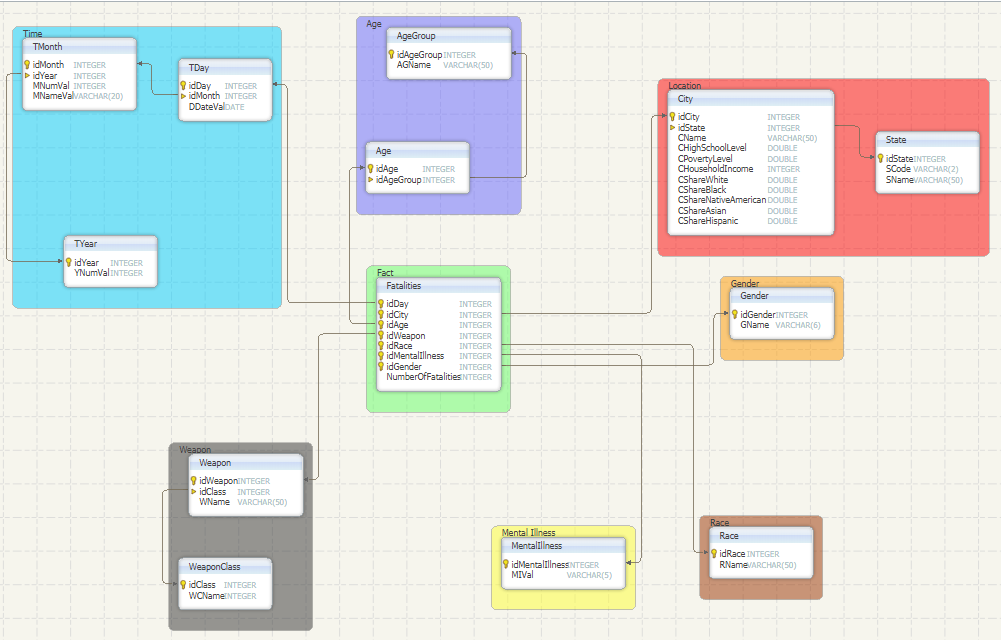
\includegraphics[width=1.0\columnwidth]{images/snapshot2}
	\caption{Overview of the CDWH}
	\label{fig:probov2}
\end{figure}
%

For the creation of the DM, 4 tables were kept exactly as the same from the CDWH: Gender, MentalIllness, Race and  Fatalities (our fact table). Each of these tables were already alone in the dimensions of the CDWH, so there was no need to aggregate their information.
The Fatalities table, which already had its data aggregated in the CDWH from 2 different tables in the Staging Area was also already prepared for the DM.  The 4 remaining dimensions were aggregated as follows: 

\begin{enumerate}
	\item Time dimension: TYear, TMonth and TDay were aggregated into Tday. 
	\item Age dimension: AgeGroup and Age were aggregated into Age.
	\item Weapon dimension: Weapon and WeaponClass were aggregated into Weapon.
	\item Location dimension: City and State were aggregated into City.
\end{enumerate}

\begin{figure}[htb]
	\centering
		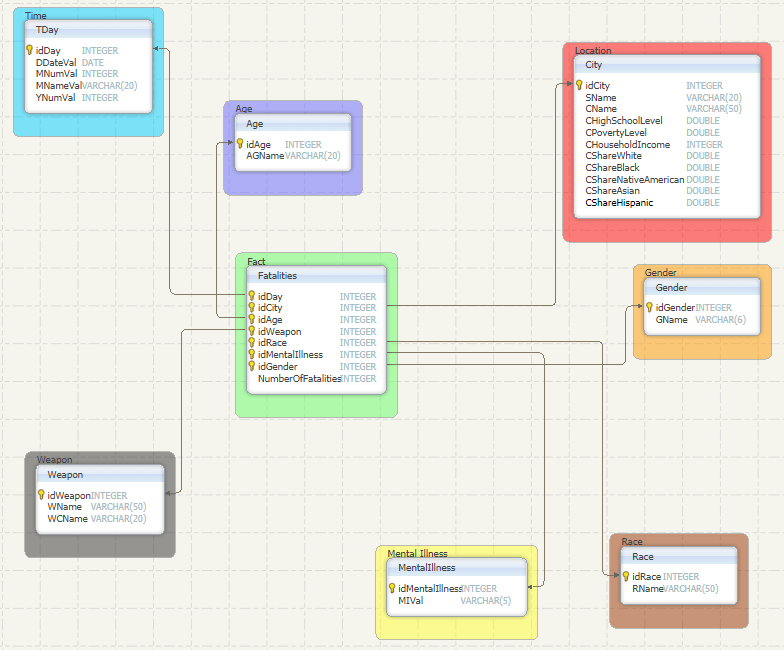
\includegraphics[width=1.0\columnwidth]{images/snapshot3}
	\caption{Overview of DM}
	\label{fig:probov}
\end{figure}
 
%%%%%%%%%%%%%%%%%%%%%%%%%%%%%%%%%%%%%%%%%%%%%%%%%%%%%%%%%%%%%%%%%%%%%%%%%%%%%%%%%%%%%%%%%%%%%%%%%%%%%%%%%%%%%%%%%%%%%%%%%%%%%%%%
%%%%%%%%%%%%%%%%%%%%%%%%%%%%%%%%%%%%%%%%%%%%%%%%%%%%%%%%%%%%%%%%%%%%%%%%%%%%%%%%%%%%%%%%%%%%%%%%%%%%%%%%%%%%%%%%%%%%%%%%%%%%%%%%
\section{Analytics} \label{sec:analytics}
Using our DM, we have created a view consisting of our fact table joined with all the other dimensions, thus creating a high-granularity table, which we exported as a CSV file and produced the following analysis plots using RStudio.

\vspace{25mm}

Data visualization:

\begin{figure}[htb]
	\centering
		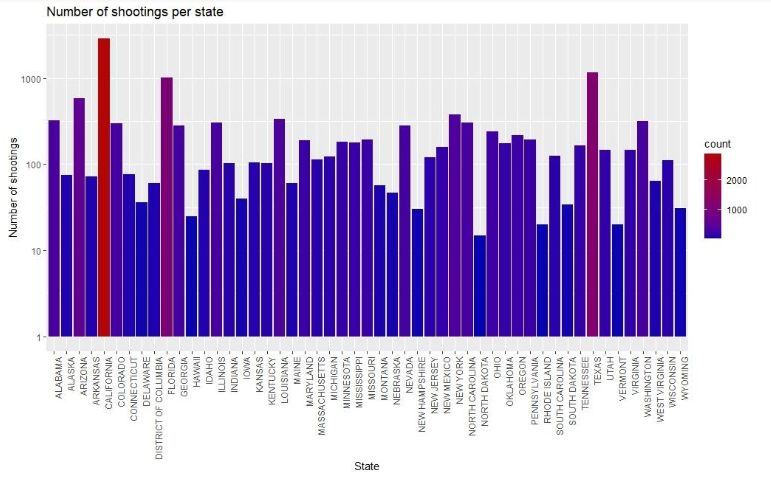
\includegraphics[width=1.0\columnwidth]{images/snapshot4}
	\caption{It is clearly shown that the states with the highest number of police fatality shootings are California, Texas, Florida, etc.}
	\label{fig:probov}
\end{figure}

\vspace{25mm}

\begin{figure}[htb]
	\centering
		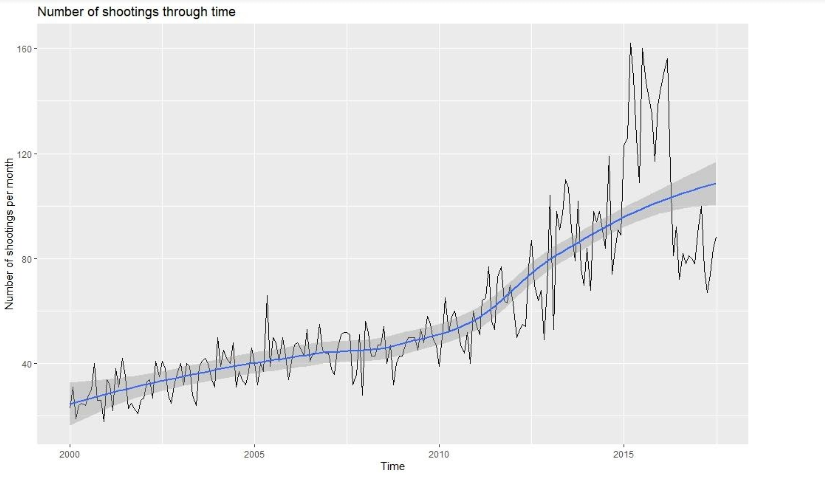
\includegraphics[width=1.0\columnwidth]{images/snapshot5}
	\caption{Monthly reported fatal police shootings have increased through time, with the biggest spike reported shortly after the 2016 presidential election.}
	\label{fig:probov}
\end{figure}

\newpage

% \begin{figure}[htb]
% 	\centering
% 		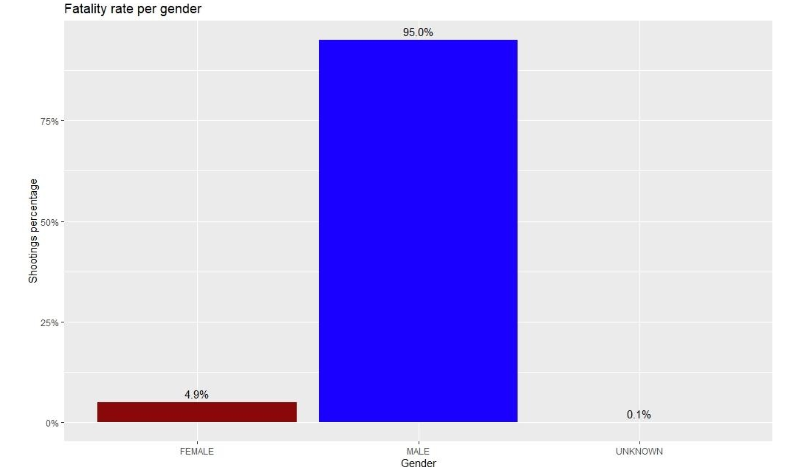
\includegraphics[width=1.0\columnwidth]{images/snapshot6}
% 	\caption{The majority of fatal police shootings include males.}
% 	\label{fig:probov}
% \end{figure}

\begin{figure}[htb]
	\centering
		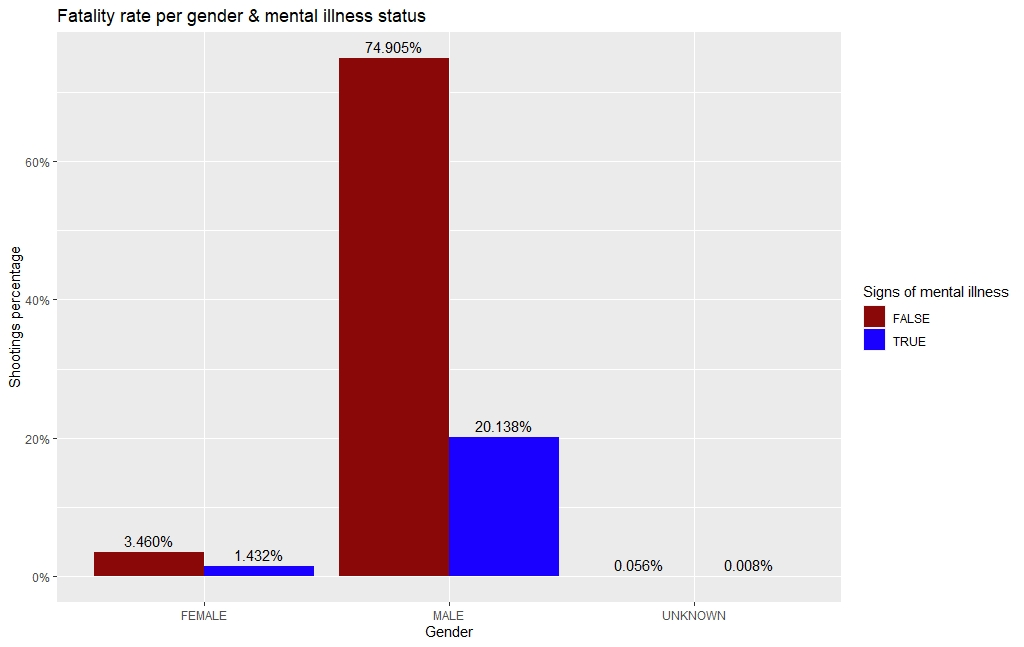
\includegraphics[width=1.0\columnwidth]{images/snapshot12}
	\caption{The majority of fatal police shootings include males and mentally health people.}
	\label{fig:probov}
\end{figure}

% \begin{figure}[htb]
% 	\centering
% 		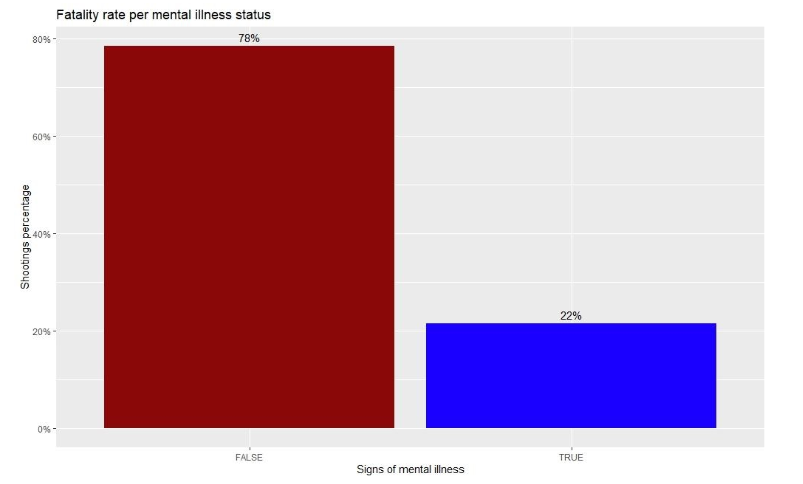
\includegraphics[width=1.0\columnwidth]{images/snapshot7}
% 	\caption{Most of the victims of fatal police shootings had no sign of mental illness.}
% 	\label{fig:probov}
% \end{figure}

\begin{figure}[htb]
	\centering
		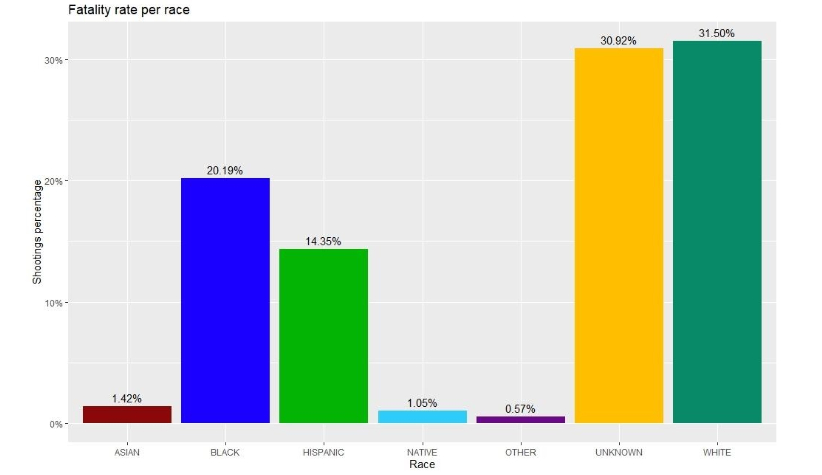
\includegraphics[width=1.0\columnwidth]{images/snapshot8}
	\caption{With ~31\% being unknown, we can’t conclude on which is the most targeted race of fatal police shootings.}
	\label{fig:probov}
\end{figure}

\begin{figure}[htb]
	\centering
		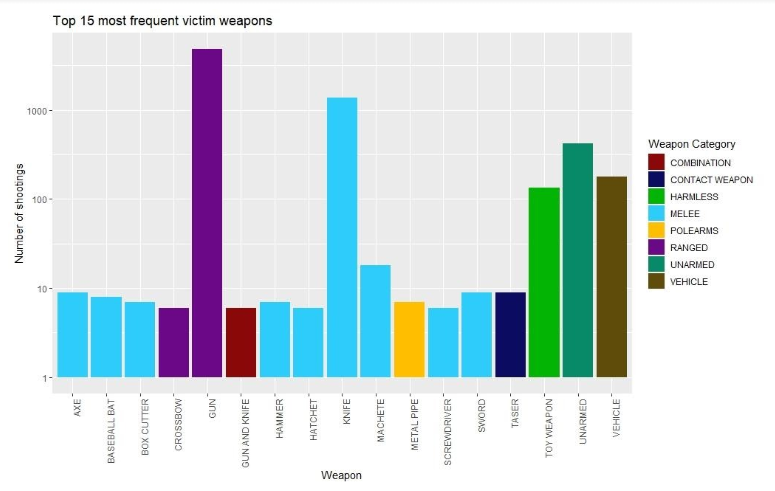
\includegraphics[width=1.0\columnwidth]{images/snapshot9}
	\caption{These are the 15 most used known weapons carried by victims of fatal police shootings.}
	\label{fig:probov}
\end{figure}

\begin{figure}[htb]
	\centering
		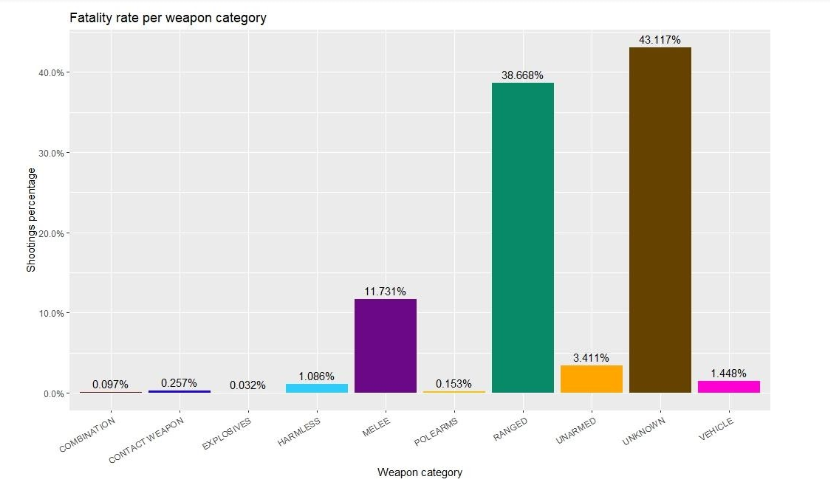
\includegraphics[width=1.0\columnwidth]{images/snapshot10}
	\caption{The majority of entries in the dataset fail to report whether a weapon was carried or not by fatal police shootings’ victims.}
	\label{fig:probov}
\end{figure}

%%%%%%%%%%%%%%%%%%%%%%%%%%%%%%%%%%%%%%%%%%%%%%%%%%%%%%%%%%%%%%%%%%%%%%%%%%%%%%%%%%%%%%%%%%%%%%%%%%%%%%%%%%%%%%%%%%%%%%%%%%%%%%%%
%%%%%%%%%%%%%%%%%%%%%%%%%%%%%%%%%%%%%%%%%%%%%%%%%%%%%%%%%%%%%%%%%%%%%%%%%%%%%%%%%%%%%%%%%%%%%%%%%%%%%%%%%%%%%%%%%%%%%%%%%%%%%%%%

\section{Conclusion} \label{sec:concl}
In this paper it was shown that:

\begin{enumerate}
	\item the number of fatal police shootings in the US:
		\begin{itemize}
 		 \item in 2017 it was 4x higher than in 2000.
 		 \item was higher for males.
 		 \item was higher for people with no sign of mental illness.
  		\item was higher for adults.  
		\item was higher for white people than other race, excluding the fact that a big percentage was not reported.
		\item included a plethora of distinct weapons with the 3 most frequent being gun, knife and unarmed.
		\end{itemize}
	\item many entries failed to report used weapon, race and age.
	\item many cities did not provide any statistics.
	\item there were many cities exclusive to one race.
	\item fatal police shootings involved 1-year-old children to 107-year-old elders.
\end{enumerate}

Further data exploration by combining dimensions can reveal more conclusions, on which specific type(s) of people were targeted in this 18-year period.

\bibliographystyle{plaindin}
\bibliography{bibliography}
\end{document}
